\section{Auswertung}
\label{sec:Auswertung}

\subsection{Bestimmung der Zeitkonstanten}

Weil das vom Oszilloskop angezeigte Bild teilweise etwas flackerte, sind zur Aufnahme der Messwerte die in \ref{fig:messA}
gezeigten Fotos aufgenommen worden. 
Hierbei wird durch Abbildung~\subref{fig:maxU_C} die Amplitude der Generatorspannung indirekt angezeigt: 
Bei niedriger Frequenz -- hier ${\SI{25.11}{\hertz}}$ -- wird der Kondensator nahezu vollständig geladen und ebenso wieder entladen. 
Somit wird eine Generatorspannung von ${U_0=\SI{4.8}{\volt}}$ abgelesen (gemäß der verwendeten Skalierung entspricht 
ein Kästchen einem Volt).

\begin{figure}
    \centering
    \begin{subfigure}{0.48\textwidth}
        \centering
        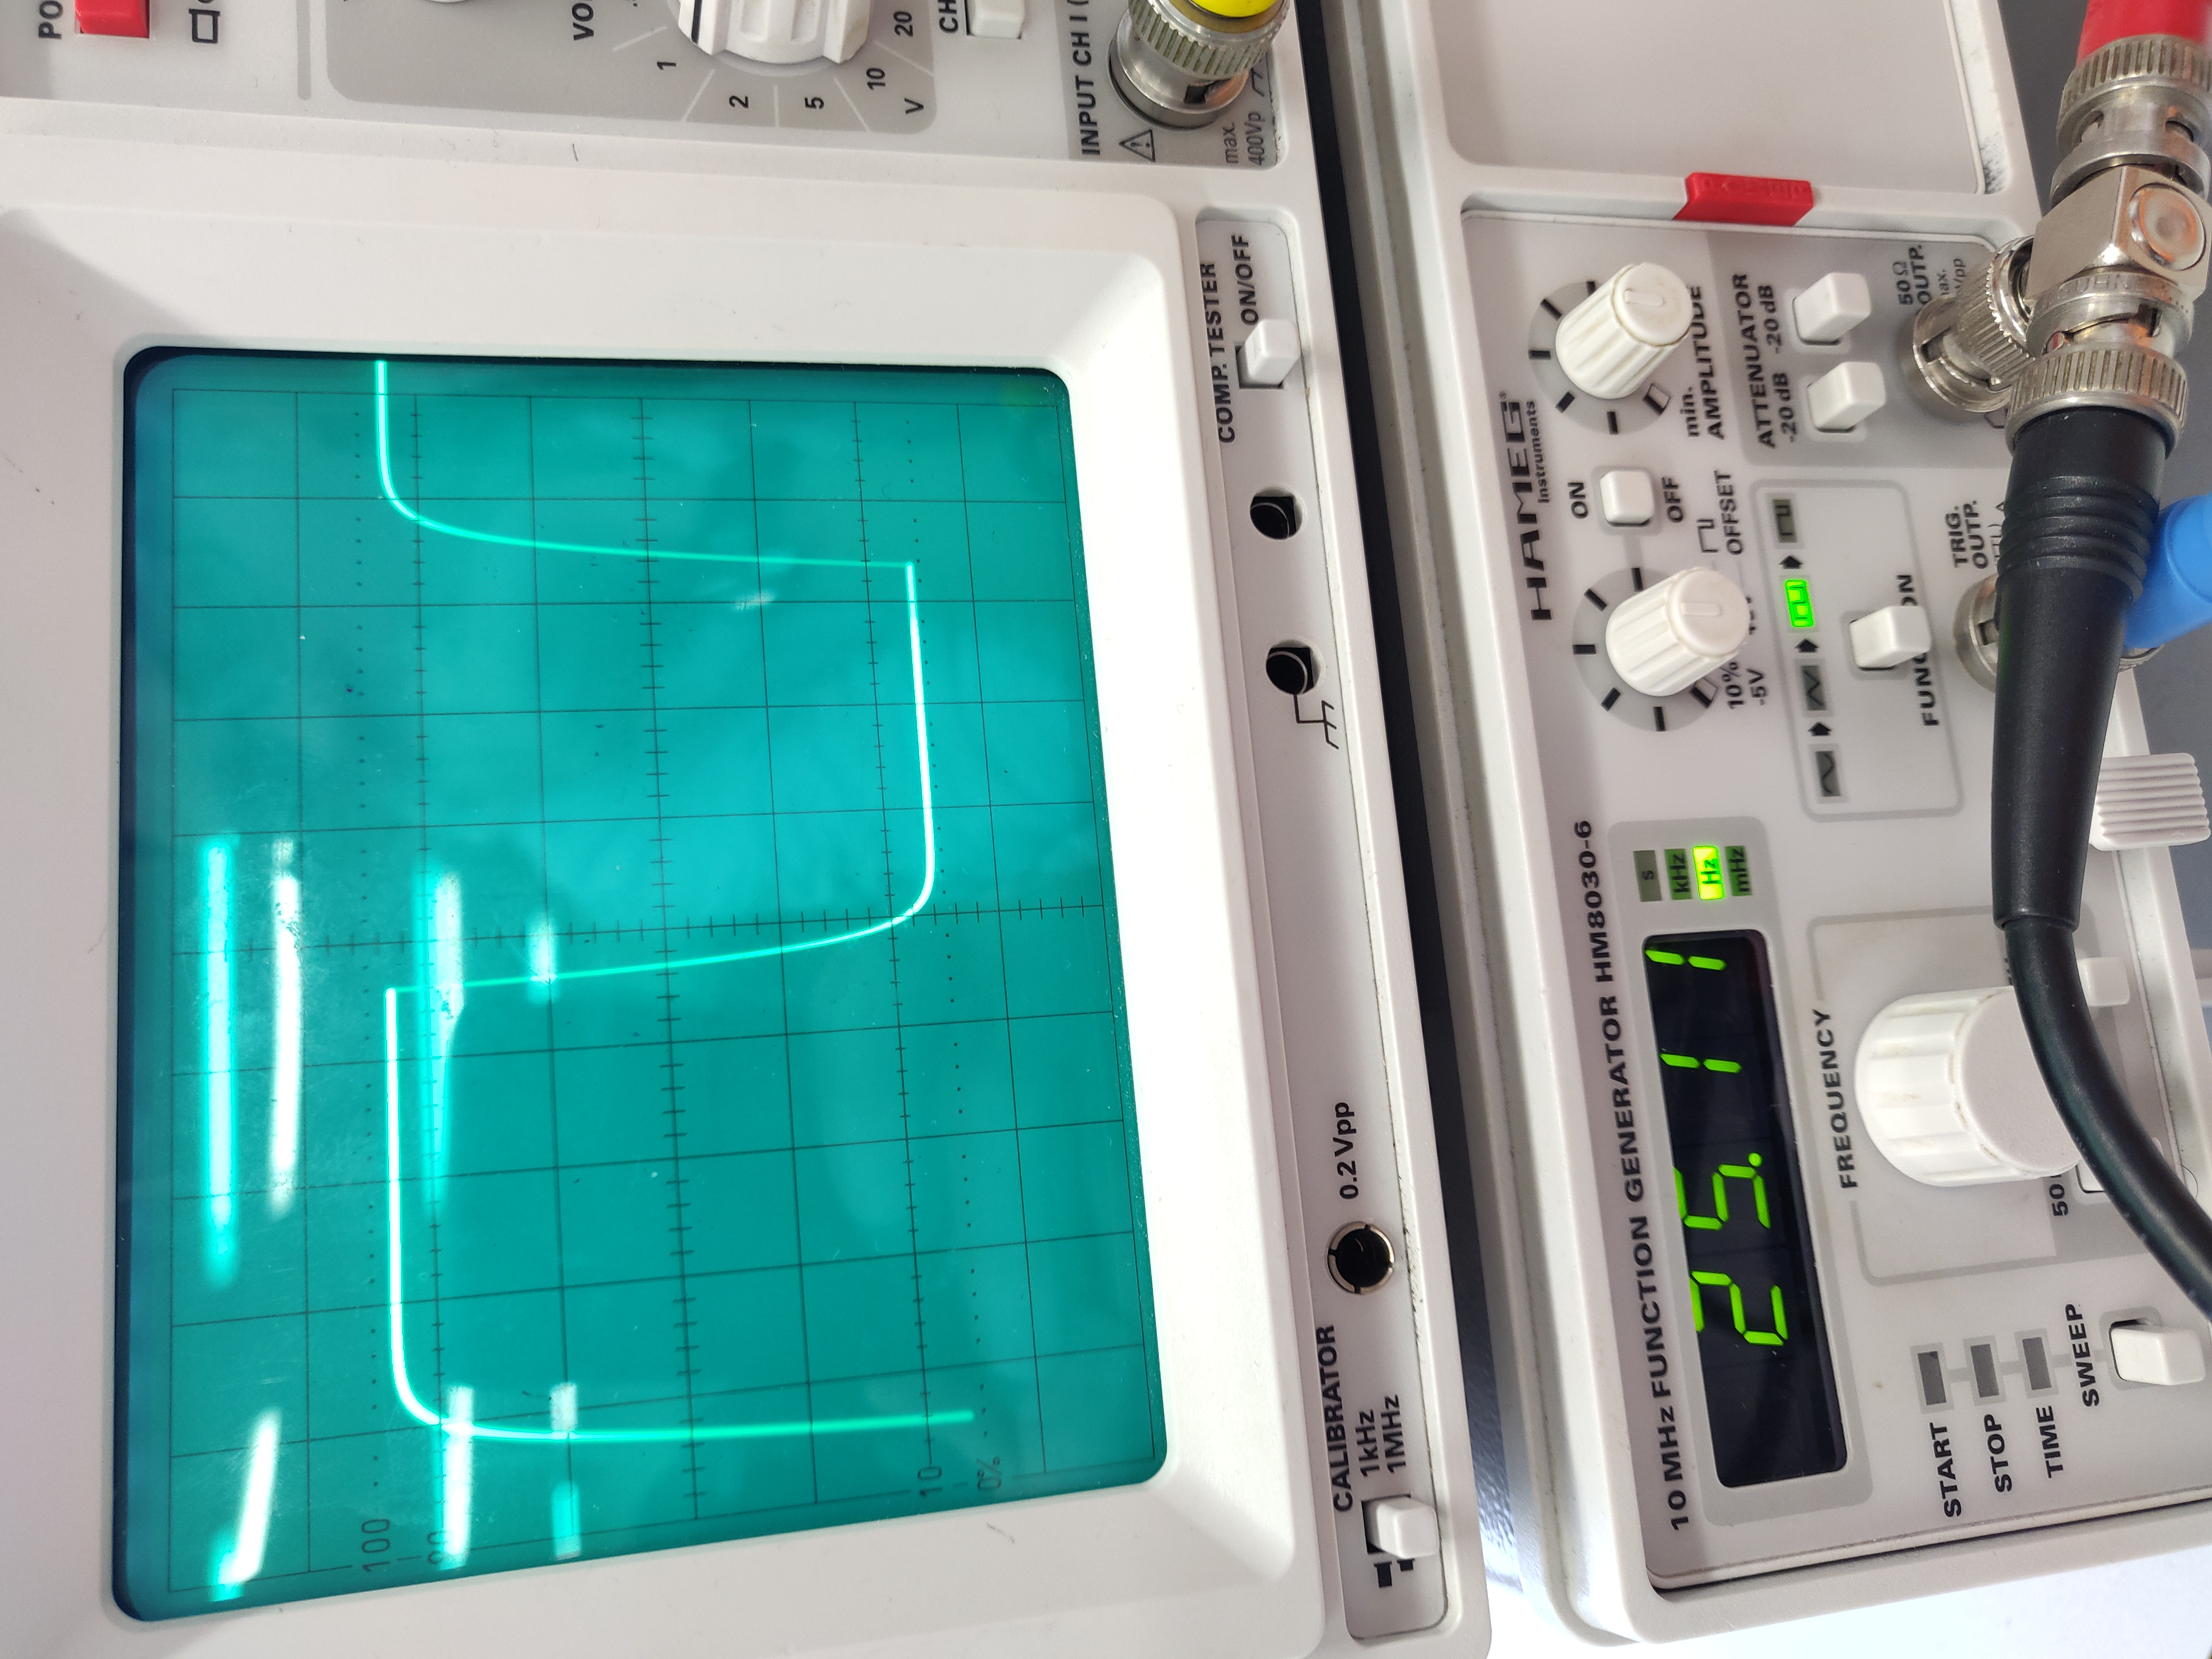
\includegraphics[height=5cm,angle=-90]{plots/maxLadungKond.jpg}
        \caption{Asymptotisch genäherte maximale Spannung des Kondensators.}
        \label{fig:maxU_C}
    \end{subfigure}
    \begin{subfigure}{0.48\textwidth}
        \centering
        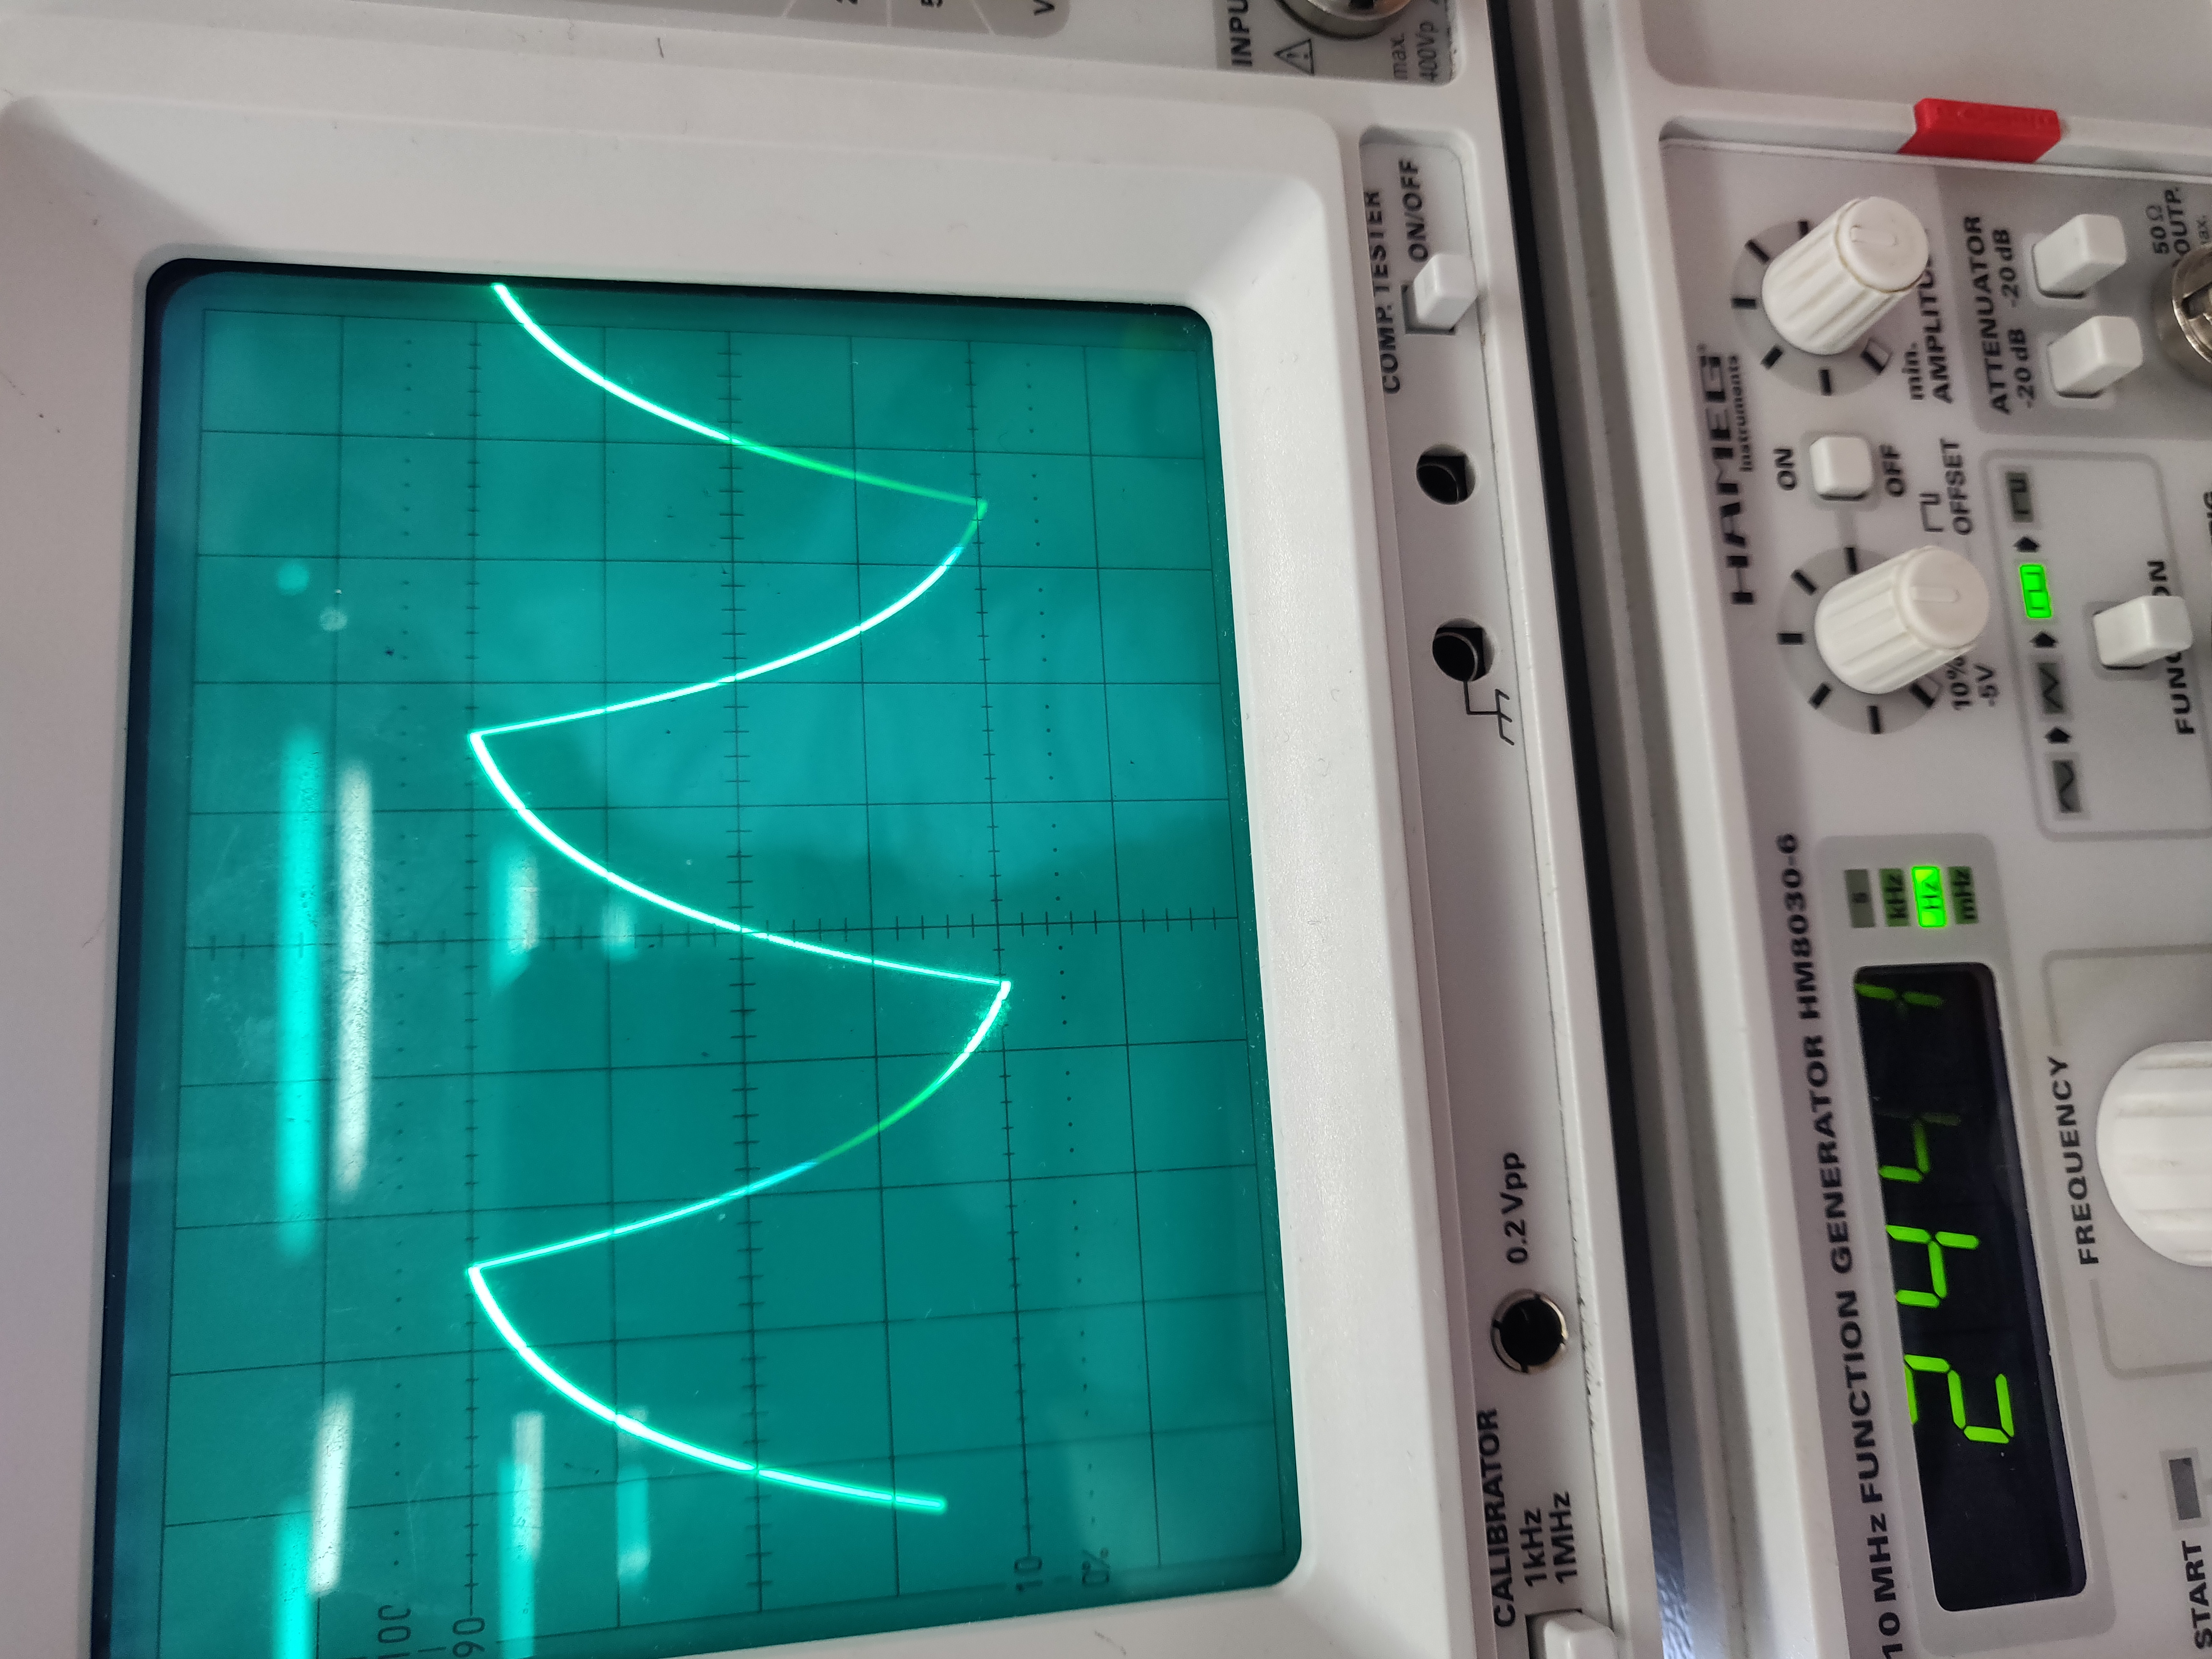
\includegraphics[height=5cm,angle=-90]{plots/LadungKondZacken.jpg}
        \caption{Zeitverlauf beim Auf- und Entladen.}
        \label{fig:UpAndDown}
    \end{subfigure}
    \caption{Verwendete Fotos zur Aufnahme der Messwerte.}
    \label{fig:messA}
\end{figure}

In \subref{fig:UpAndDown} beläuft sich eine Periodendauer auf genau vier Kästchen auf der Zeitachse. 
Mit der Frequenz ${f=\SI{244.1}{\hertz}}$ und $T=\sfrac{1}{f}$ kann eine entsprechende Relation zwischen der Anzahl der Kästchen und der 
Zeit $t$ hergestellt werden. 

\begin{table}
    \centering
    \label{tab:Aaa}
    \caption{Messwerte zur Bestimmung der Zeitkonstanten $\tau$.}
    \begin{tabular}{S[table-format=1.1] S[table-format=1.3] S[table-format=1.2]}
        \toprule
        {Anzahl Kästchen (Zeit)} & {$t\:/\:\SI{e-3}{\second}$} & {$U_C\:/\:\si{\volt}$} \\
        \midrule
        -2.4 & -2.458 & 4.35    \\
        -2.2 & -2.253 & 3.2     \\
        -2.0 & -2.048 & 2.6     \\
        -1.8 & -1.843 & 2.0     \\
        -1.6 & -1.638 & 1.6     \\
        -1.4 & -1.434 & 1.2     \\
        -1.2 & -1.229 & 0.9     \\
        -1.0 & -1.024 & 0.7     \\
        -0.8 & -0.819 & 0.55    \\
        -0.6 & -0.614 & 0.48    \\
        -0.4 & -0.410 & 0.35    \\
        \bottomrule
    \end{tabular}
\end{table}

In Tabelle 1 %\ref{tab:Aaa} ich habe wirklich keine Ahnung, warum die Referenz hier nicht funktioniert
 sind die entsprechenden Messwerte aufgeführt, die für die folgende Ausgleichsrechnung verwendet werden. 
Wie in \ref{sub:AufUndAb} geschildert, verhält sich die Spannung eines Kondensators beim Entladen gemäß 
\begin{equation}
    U_C(t)=U_0 \exp(-\frac{1}{RC}(t-B))\:.
\end{equation}
Durch Ausgleichsrechnung mithilfe von \textit{Python 3.7.3} werden die Konstanten $A$ und $B$ von der Gerade
%Konstante B ist nötig, da die Kurve, die wir vermessen haben, ja nicht bei -2.458*10^-3 s ihr Maximum von U_0 erreicht, sondern nur 90% dessen o.ä... 
%also B ist nur zur Verschiebung der Gerade da.
\begin{equation}
    (\ln{U_C})(t) = \ln{U_0} -\frac{1}{RC}(t-B) =: \ln{U_0} -A(t-B)
    \label{eqn:gerade} %U_0=4.8Volt
\end{equation} 
bestimmt. $B$ wird hier für die Verschiebung der Gerade benutzt, da bei ${t=\SI{0}{\second}}$ der Kondensator im Experiment 
keine Spannung von $U_0$ erreicht. 
\begin{gather}
    y=a\cdot x + b \\
    y \,\widehat{=}\, \ln{U_C} \,, \quad
    x \,\widehat{=}\, t\,, \\
    a \,\widehat{=}\,-A=-\frac{1}{RC}=-\frac{1}{\tau} \,, \quad
    b \,\widehat{=}\, \ln{U_0} +B\cdot A = \ln{U_0} +B\cdot \frac{1}{RC} \\
    \Rightarrow 
    \tau=RC=\frac{1}{A}=\SI{0.82(1)e-3}{\second} \,, \quad 
    B=\SI{-2.56(5)e-3}{\second} 
\end{gather}

Die Messwerte inklusive der Geraden \eqref{eqn:gerade} sind in \ref{fig:ausgl_gr_A} 
mit der entsprechenden Achsenskalierung aufgetragen. 

\begin{figure}
    \centering
    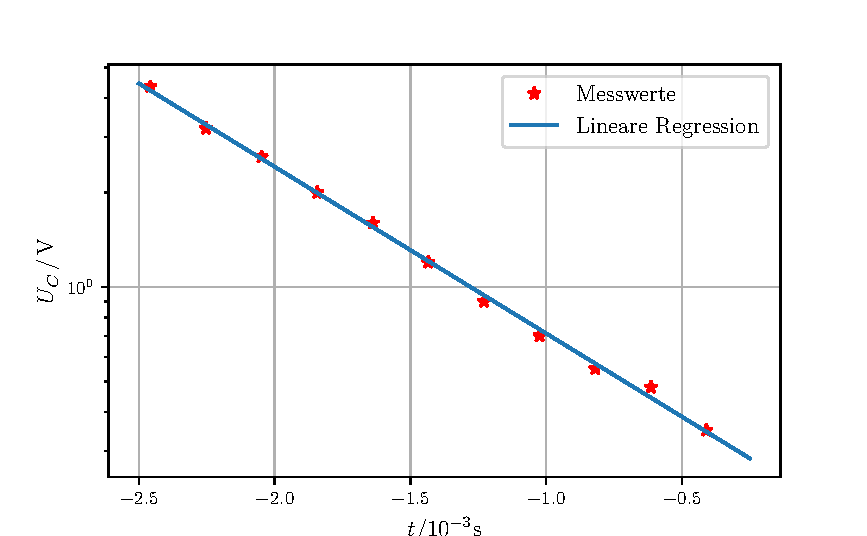
\includegraphics[width=0.9\textwidth]{plots/ausgleichsgerade.pdf}
    \caption{Die Messwerte und die zugehörige Ausgleichsgerade der ersten Messung.}
    \label{fig:ausgl_gr_A}
\end{figure}

Dem aus dem Experiment bestimmten Wert für die Zeitkonstante $\tau$ kann der theoretisch zu erwartende Wert gegenübergestellt werden. 
Die Referenzbauteile haben die Kenngrößen ${R=\SI{15.058(600)}{\kilo\ohm}}$ und ${C=\SI{93.3}{\nano\farad}}$. 
Daraus ergibt sich die theoretische Zeitkonstante zu $\tau _\text{theo}=\SI{1.405(56)}{\milli\second}$.

\FloatBarrier

\subsection{Frequenzabhängigkeit der Amplitude und der Phasenverschiebung}
 
%Der Generator hatte eine Spannung von 2.7 Volt

Die Messungen der Amplituden und Phasenverschiebungen werden parallel aufgenommen. Für jede Frequenz ergibt sich also ein Wertepaar.
Das Oszilloskop wird so kalibriert, dass ein vertikales Kästchen $= \SI{1}{\volt}$ entspricht. Die Auflösung der Zeitachse ist irrelevant, da nur die Verhältnisse von Bedeutung sind.
Die Amplitude der Generatorspannung liegt bei allen Messwerten bei $\SI{2.7}{\volt}$, also $2.7$ Kästchen, wie in Abbildung \ref{fig:methodik} zu sehen ist.

\begin{figure}
    \centering
    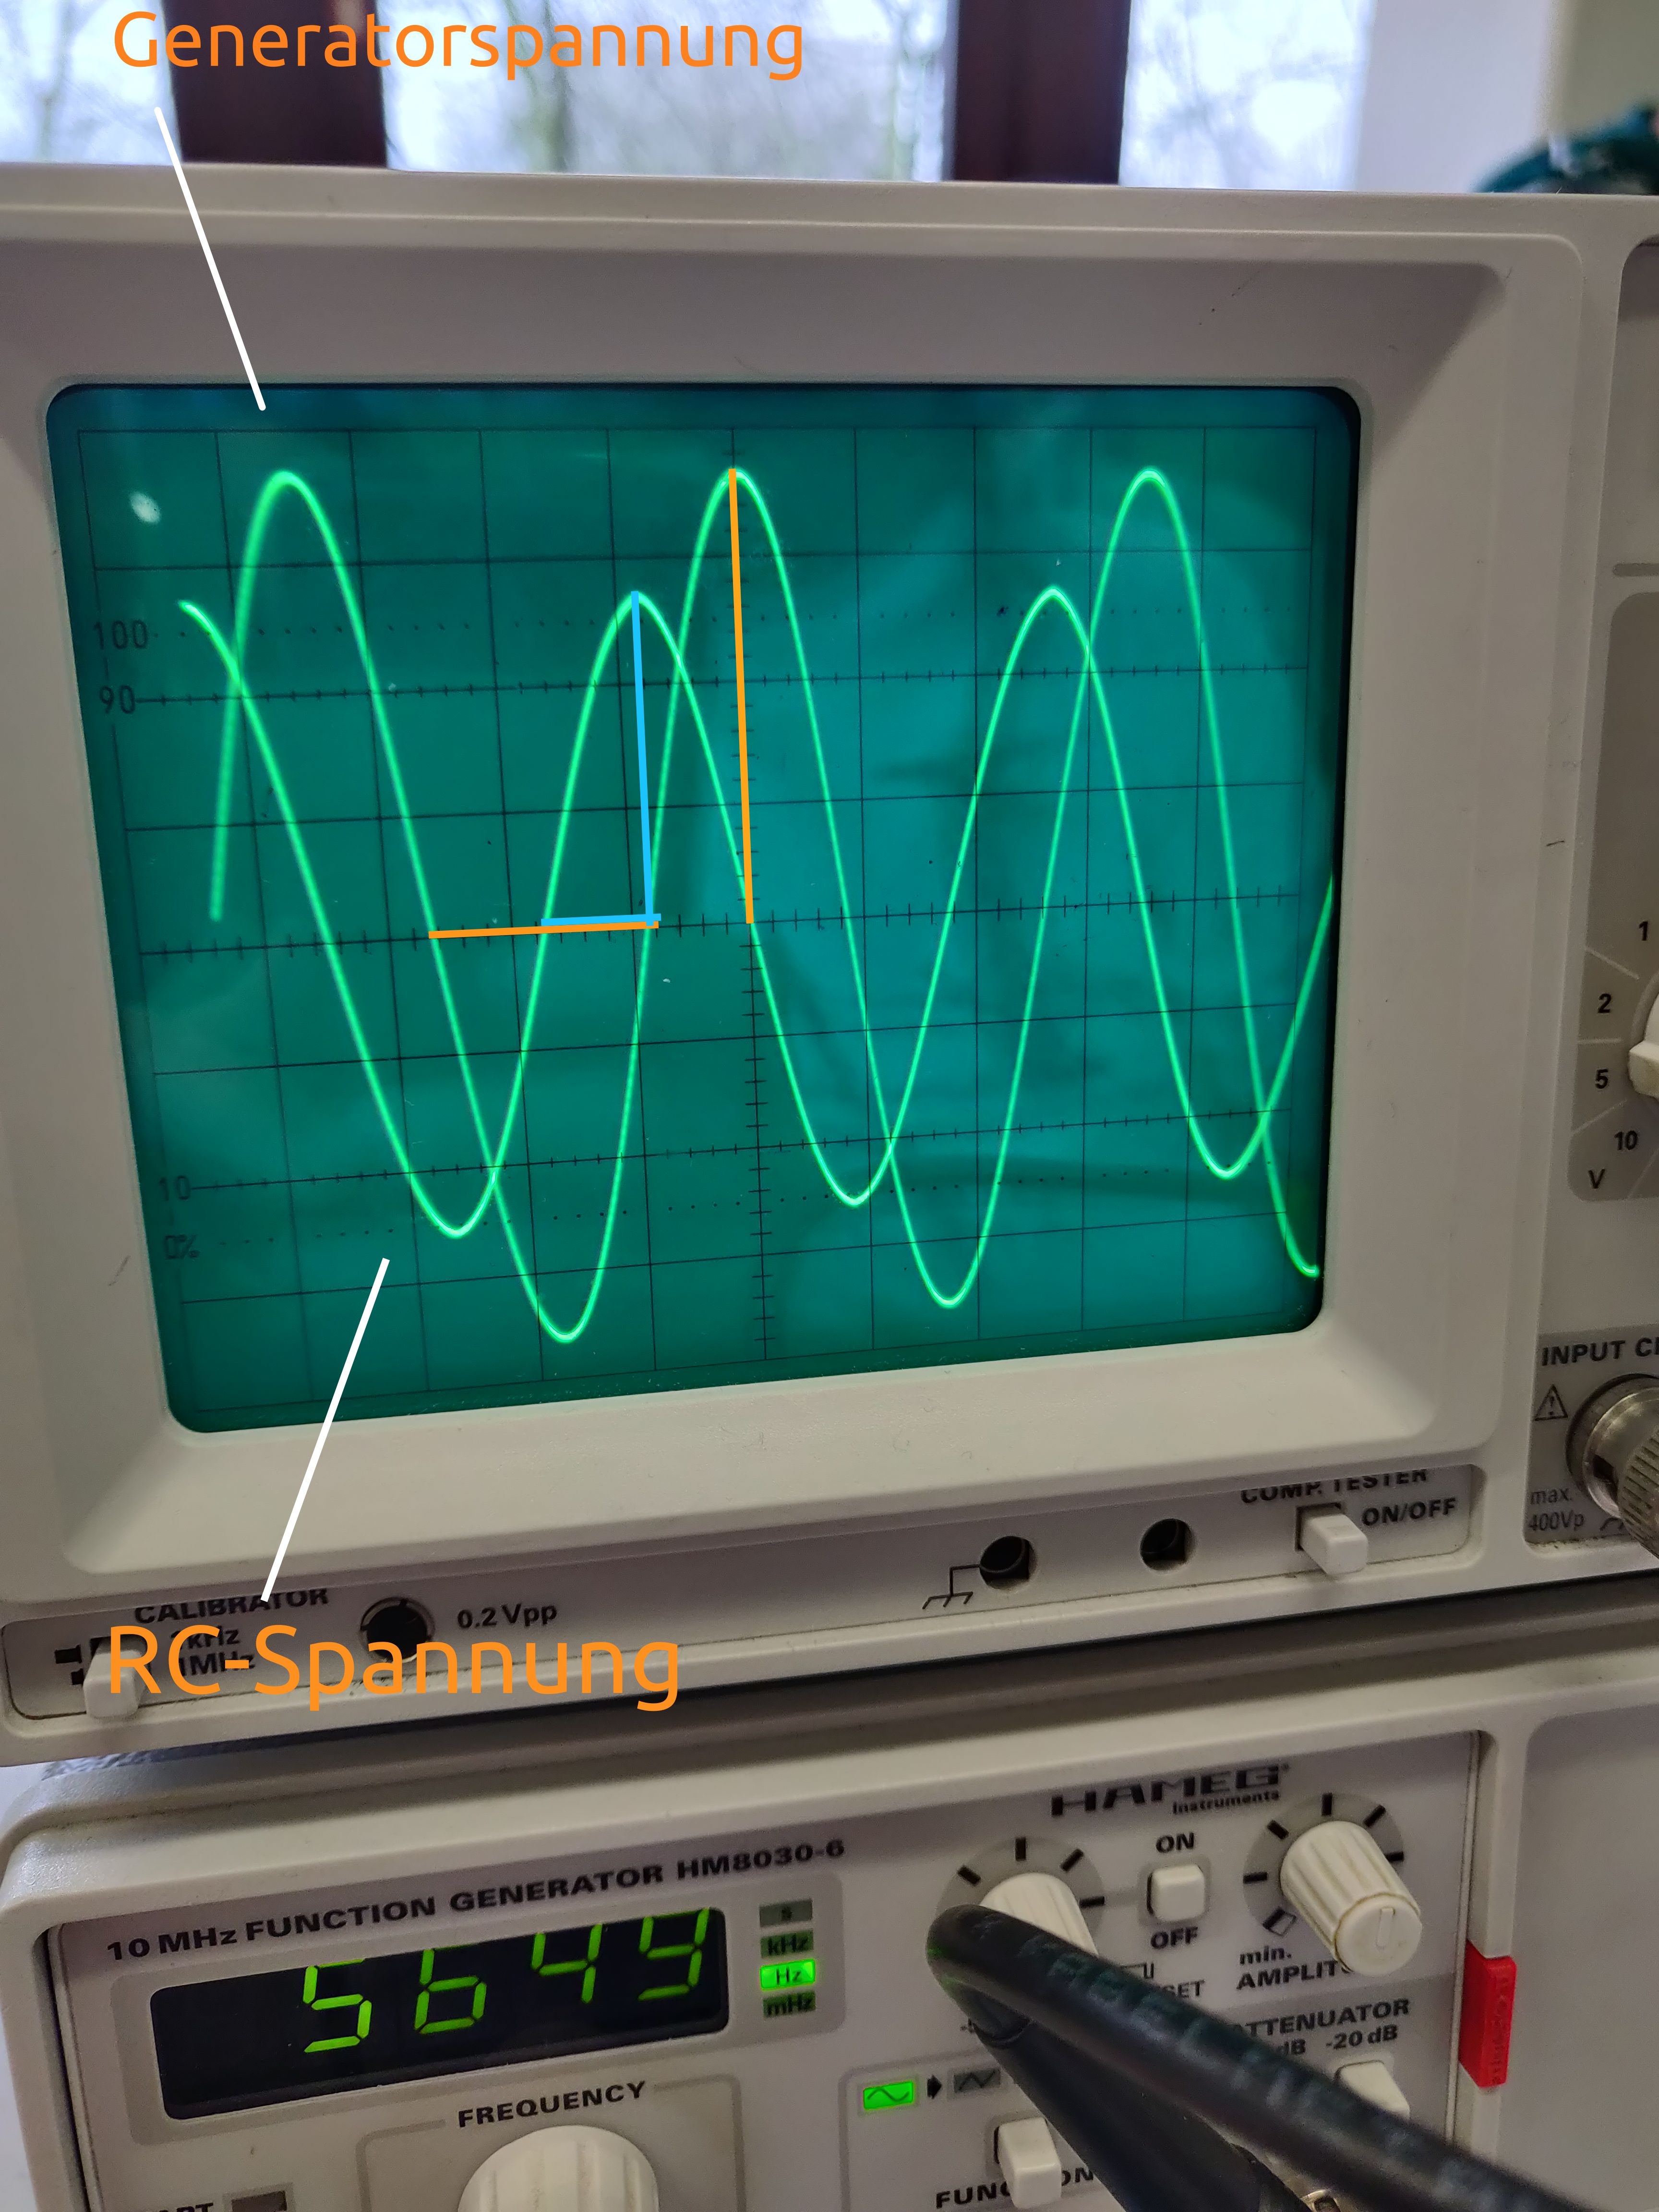
\includegraphics[width=0.8\textwidth]{plots/beispiel_Messung.jpg}
    \caption{Methodik der Messwertaufnahme.}
    \label{fig:methodik}
\end{figure}

Für die Phasenverschiebung wird das Verhältnis der horizontalen Linien bestimmt, wobei Orange die Generatorspannung darstellt. Durch diese Methode ergibt sich direkt ein Wert als Bruchteil von $\pi$.
Entsprechend werden für die Amplituden die vertikalen Linien verglichen.
Für die in \ref{sec:durch_freq} beschriebenen Messungen der drei Größenordnungen ergeben sich die Werte in den Tabellen \ref{tab:BbbCcc1} und \ref{tab:BbbCcc23}.

\begin{table}
    \centering
    \caption{Messung in der kleinsten Größenordnung.}
    \label{tab:BbbCcc1}
    \begin{tabular}{S[table-format=3.2] S[table-format=1.2] S[table-format=1.3]}
        \toprule
        {$f\:/\:\si{\hertz}$} & {$U\:/\:\si{\volt}$} & {$\increment \varphi\:/\:\symup{\pi}$} \\
        \midrule
        15.25 & 2.50 & 0.035 \\
        20.50 & 2.50 & 0.037 \\
        23.25 & 2.50 & 0.050 \\
        26.65 & 2.50 & 0.047 \\
        30.20 & 2.50 & 0.051 \\
        39.50 & 2.45 & 0.067 \\
        45.40 & 2.50 & 0.077 \\
        57.25 & 2.40 & 0.092 \\
        63.50 & 2.40 & 0.098 \\
        71.40 & 2.39 & 0.112 \\
        76.20 & 2.36 & 0.120 \\
        80.40 & 2.34 & 0.127 \\
        85.60 & 2.30 & 0.132 \\
        92.60 & 2.24 & 0.143 \\
        99.90 & 2.22 & 0.151 \\
        108.2 & 2.20 & 0.157 \\
        112.1 & 2.18 & 0.169 \\
        121.7 & 2.12 & 0.179 \\
        125.0 & 2.10 & 0.187 \\
        131.3 & 2.09 & 0.193 \\
        \bottomrule
    \end{tabular}
\end{table}

\begin{table}
    \centering
    \caption{Messungen in den beiden größeren Größenordnungen.}
    \label{tab:BbbCcc23}
    \begin{tabular}{S[table-format=3.1] S[table-format=1.2] S[table-format=1.3]}
        \toprule
        {$f\:/\:\si{\hertz}$} & {$U\:/\:\si{\volt}$} & {$\increment \varphi\:/\:\symup{\pi}$} \\
        \midrule
        184.8 & 1.82 & 0.243 \\
        216.8 & 1.68 & 0.265 \\
        250.0 & 1.58 & 0.256 \\
        284.0 & 1.42 & 0.296 \\
        310.8 & 1.35 & 0.300 \\
        347.5 & 1.23 & 0.337 \\
        378.6 & 1.16 & 0.340 \\
        414.1 & 1.08 & 0.365 \\
        442.7 & 1.01 & 0.353 \\
        476.2 & 0.97 & 0.354 \\
        507.7 & 0.92 & 0.362 \\
        531.5 & 0.88 & 0.366 \\
        556.6 & 0.85 & 0.369 \\
        599.0 & 0.80 & 0.385 \\
        \bottomrule
    \end{tabular}
    $\qquad \qquad$
    \begin{tabular}{S[table-format=4.0] S[table-format=1.2] S[table-format=1.3]}
        \toprule
        {$f\:/\:\si{\hertz}$} & {$U\:/\:\si{\volt}$} & {$\increment \varphi\:/\:\symup{\pi}$} \\
        \midrule
        699  & 0.68 & 0.400 \\
        791  & 0.60 & 0.413 \\
        892  & 0.55 & 0.415 \\
        1020 & 0.48 & 0.422 \\
        1111 & 0.43 & 0.423 \\
        1222 & 0.40 & 0.421 \\
        1333 & 0.38 & 0.429 \\
        1444 & 0.35 & 0.426 \\
        1555 & 0.32 & 0.436 \\
        1666 & 0.29 & 0.432 \\
        1777 & 0.25 & 0.446 \\
        1888 & 0.23 & 0.436 \\
        1999 & 0.22 & 0.424 \\
        2112 & 0.21 & 0.432 \\
        \midrule
        5701 & 0.07 & 0.438 \\
        \bottomrule
    \end{tabular}
\end{table}

\FloatBarrier

Als Referenzwert wird noch eine Messung bei $\approx \SI{5700}{\hertz}$ abgelesen, welche am Ende der Tabelle \ref{tab:BbbCcc23} abzulesen ist.
In Abbildung \ref{fig:mess_b_c} sind die Messwerte eingetragen und der exponentielle Verlauf dargestellt.
Hierbei wird die Y-Achse für die Phasenverschiebung als $\Delta\varphi\:/\:\pi$ gewertet.

\begin{figure}
    \centering
    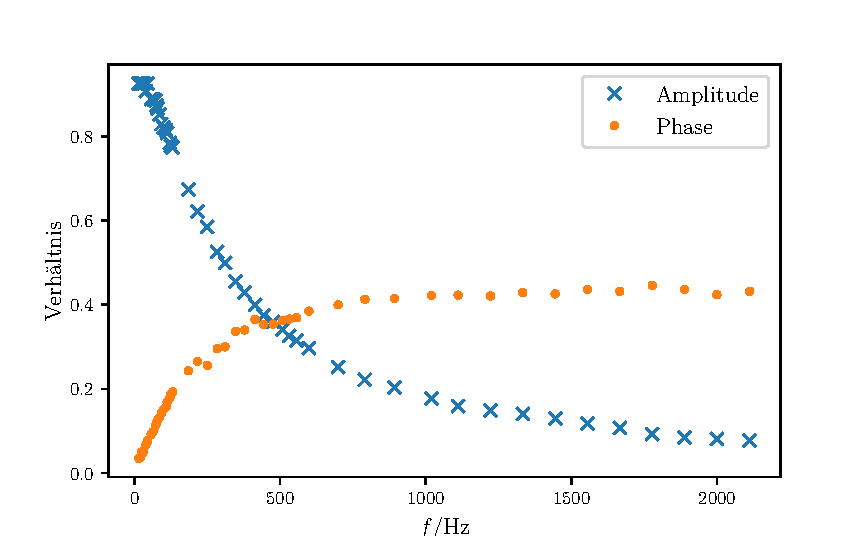
\includegraphics[width=0.8\textwidth]{plots/plot_b_c.pdf}
    \caption{Messwerte der Amplituden und Phasenverschiebungen.}
    \label{fig:mess_b_c}
\end{figure}

\subsection{Der RC-Kreis als Integrator}

Dieser Part ist wie in \ref{sec:Durchführung} beschrieben durchgeführt worden. 
Dafür wird wegen der in \ref{sec:Theorie} erläuterten analytischen Zusammenhänge eine möglichst hohe Frequenz eingestellt, 
damit der RC-Kreis die Generatorspannung um $\sfrac{\pi}{2}$ versetzt auf dem Oszilloskop ausgeben kann. 
Das Ergebnis auf dem Oszilloskop ist erneut mit der Kamera festgehalten, wie aus den Abbildungen \ref{fig:int_sinus} und 
\ref{fig:rechtdrei} \subref{fig:int_rechteck}, \subref{fig:int_dreieck} ersichtlich ist. 

Angemerkt sei noch, dass die Amplituden der beiden Spannungen unterschiedlich skaliert sind, weil die bei hoher Frequenz 
beim Kondensator ankommende Spannung sehr viel geringer ist als die Generatorspannung. 
Das an den Abbildungen zu Betrachende ist demnach ausschließlich der Verlauf und die Phasenverschiebung der Spannungskurven. 

\begin{figure}
    \centering
    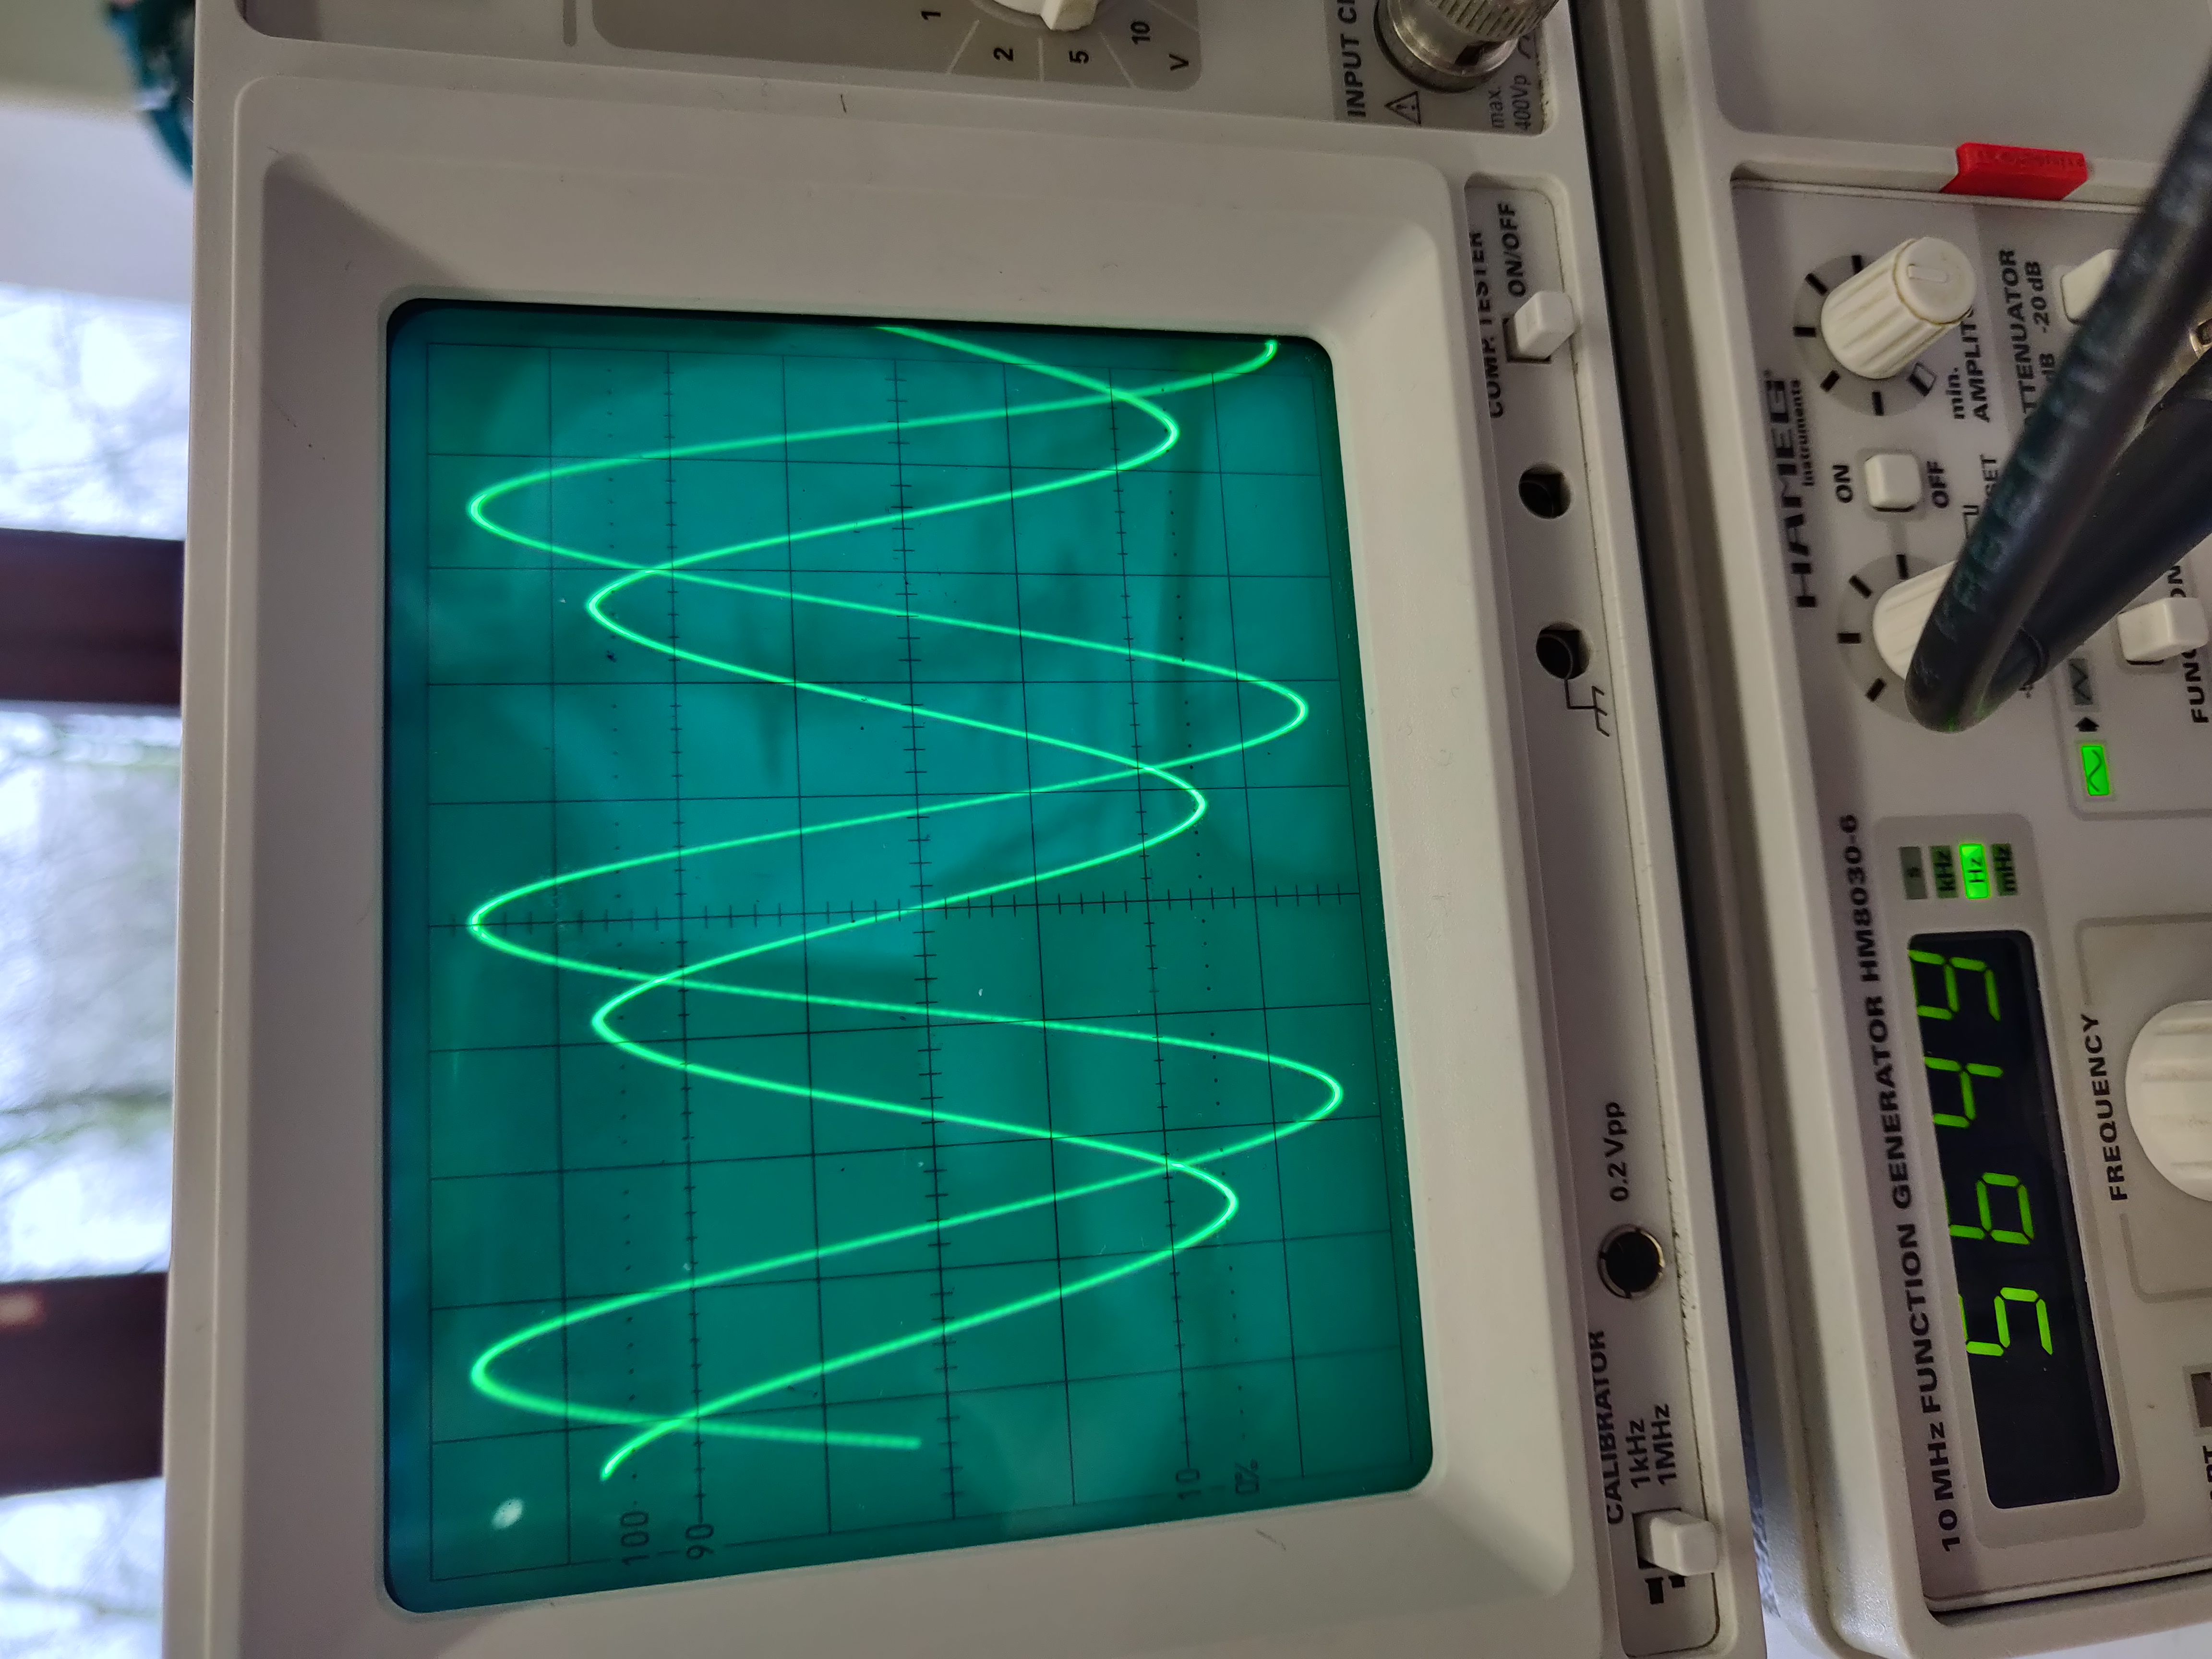
\includegraphics[angle=-90,width=0.6\textwidth]{plots/sinus.jpg}
    \caption{Die integrierte Spannung einer Sinusspannung.}
    \label{fig:int_sinus}
\end{figure}

\begin{figure}
    \centering
    \begin{subfigure}{0.48\textwidth}
        \centering
        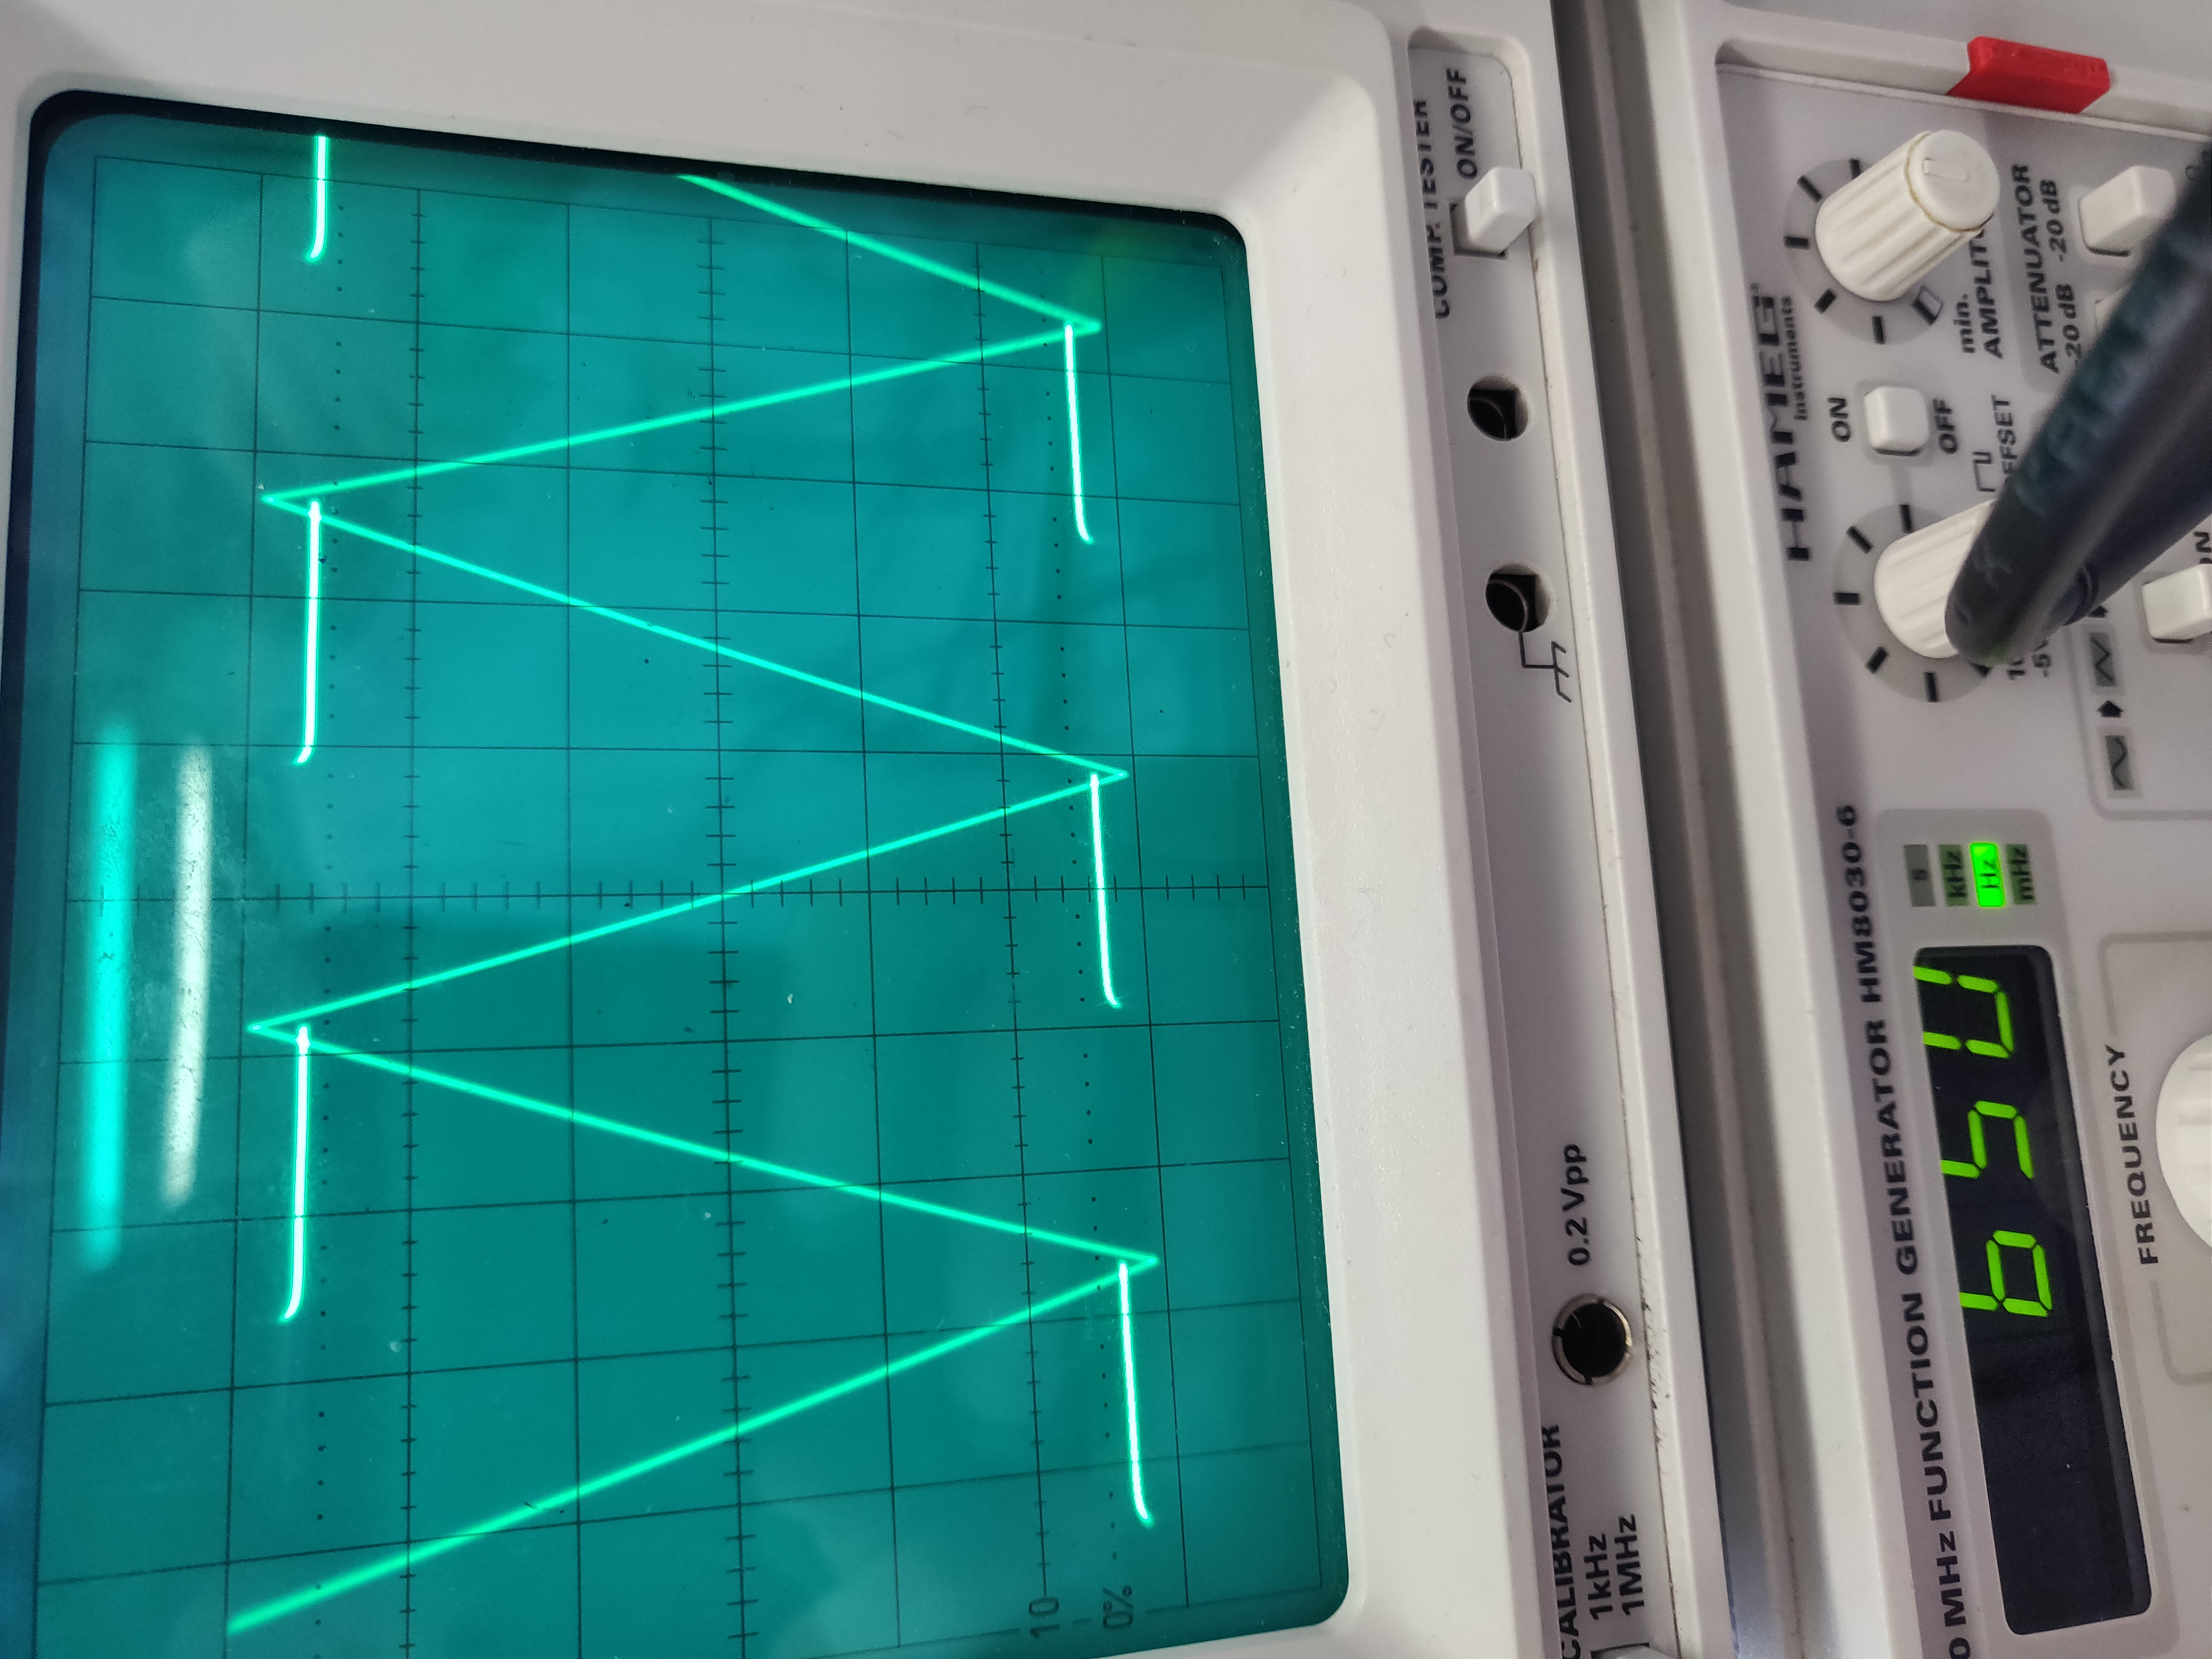
\includegraphics[height=6cm,angle=-90]{plots/rechteck.jpg}
        \caption{Die integrierte Spannung einer Rechtecksspannung.}
        \label{fig:int_rechteck}
    \end{subfigure}
    \begin{subfigure}{0.48\textwidth}
        \centering
        \includegraphics[height=6cm,angle=-90]{plots/dreieck.jpg}
        \caption{Die integrierte Spannung einer Dreiecksspannung.}
        \label{fig:int_dreieck}
    \end{subfigure}
    \caption{Die Rechtecks- und Dreicksspannung.}
    \label{fig:rechtdrei}
\end{figure}
